\documentclass[12pt,a4paper]{article}
\usepackage[a4paper, total={160mm, 242mm}]{geometry}
\usepackage{pdfpages}

%% Vytváříme PDF/A-2u
\usepackage[a-2u]{pdfx}

%% Přepneme na českou sazbu a fonty Latin Modern
\usepackage[czech]{babel}
\usepackage{lmodern}
\usepackage[T1]{fontenc}
\usepackage{textcomp}

\begin{document}
Tímto dik Pétě za zpracovaný první dva okruhy.
\includepdf[pages=-]{1-2Okruhy/statniceOM12okruhy.pdf}
\includepdf[pages=-]{3cOkruh/prace.pdf}
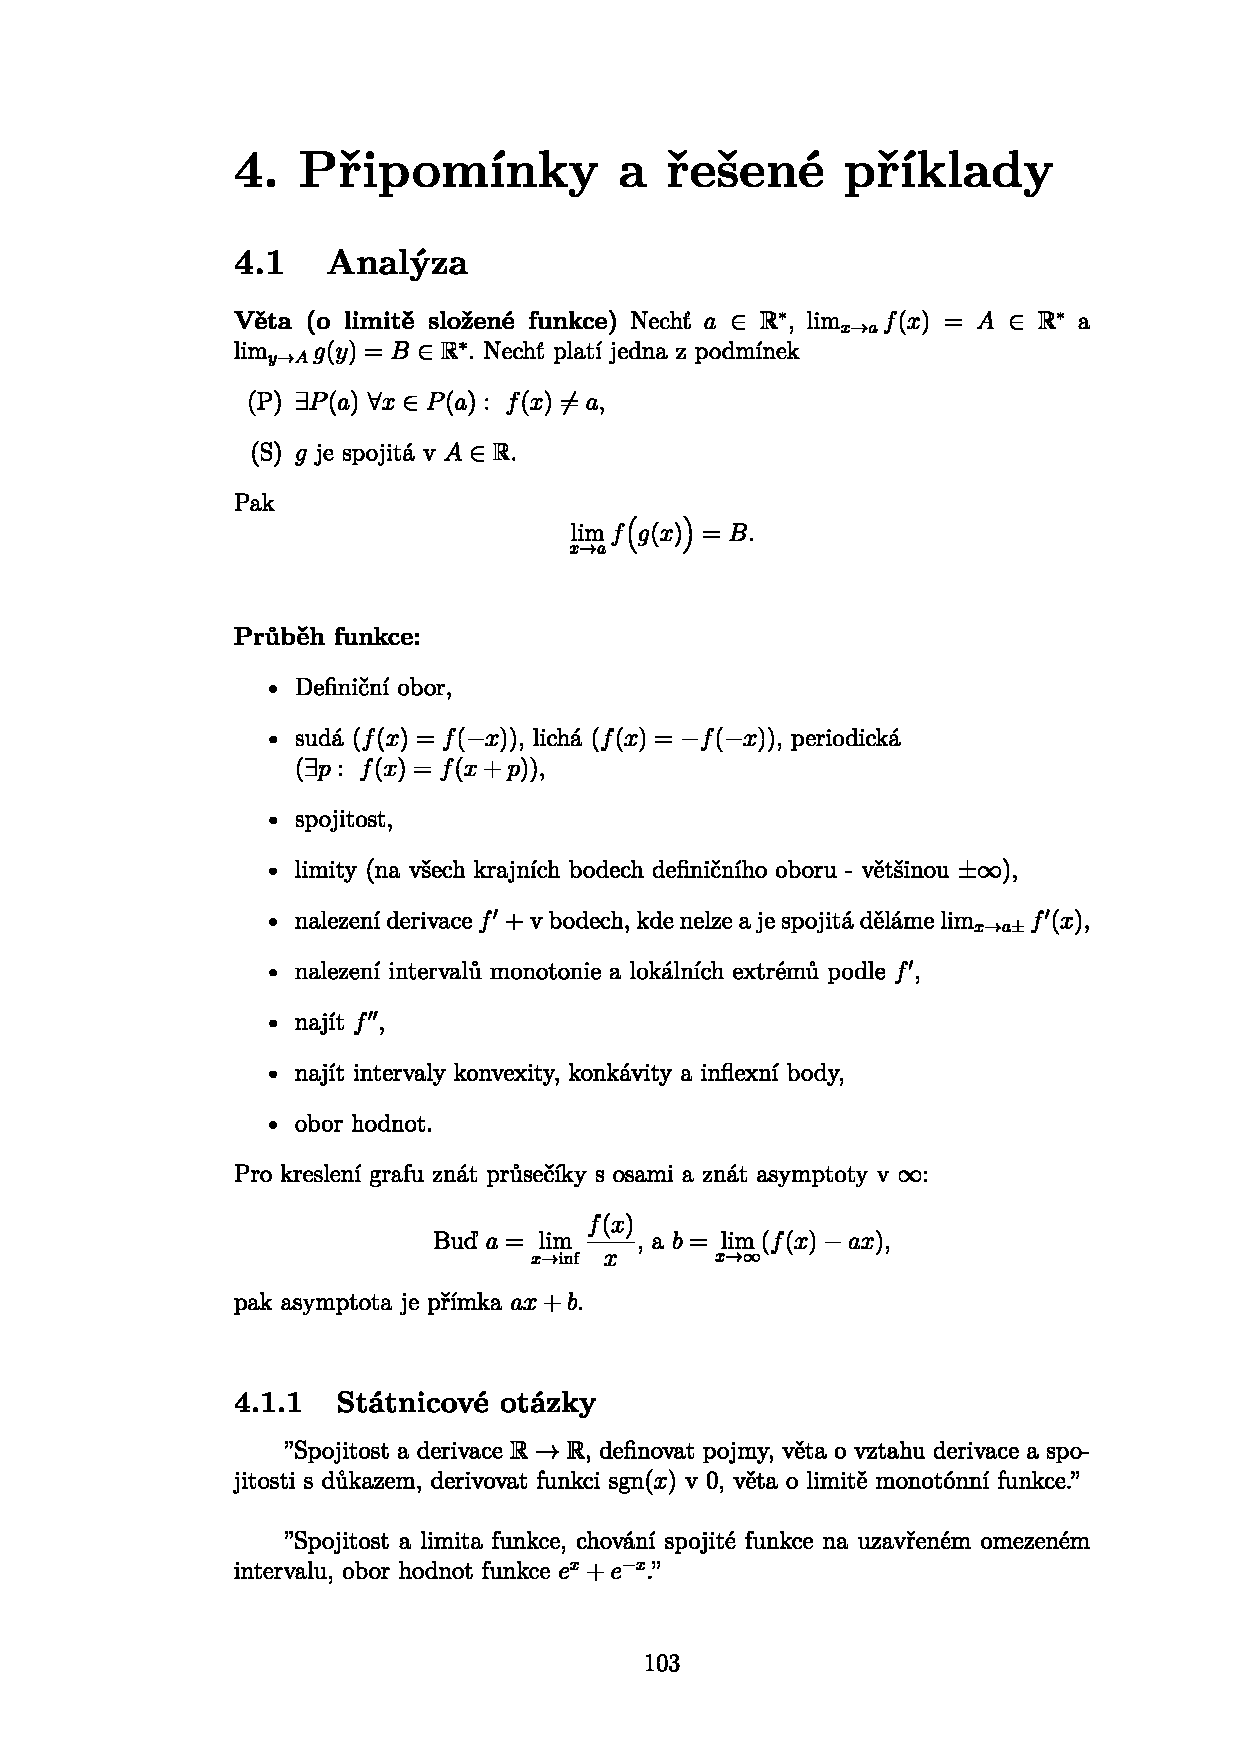
\includepdf[pages=-]{1-2Okruhy/statniceOMotazky.pdf}
\section*{Komenty k SZZ 2020}
Sesbíral jsem troje pohledy na szz, snad vám pomůžou udělat si obrázek.
\subsection*{První}
SZZ 2.7.

PRŮBĚH:

Na prezentaci je tak 10 minut ale Pick to hodně hlídal a i upozorňoval pokud někdo přetáhl. Po prezentaci se přečtou posudky a pak je prostor k vyjádření k posudkům a diskuze, většinou se někdo z komise na něco zeptá. 
Pak jdou studenti ven a komise se poradí, pak se vrátí a řeknou se výsledky. Následuje krátká přestávka a po ní nastupuje první trojice.
Každý z trojice dostane jednu otázku z nějakého okruhu a má 20 minut na potítko. Po 20ti minutách přijde další trojice a ti si opět vyberou otázky a začnou si je zpracovávat. Mezitím se zkouší ta první trojice.
Bylo nás 5 za hodinu a dvacet minut jsme byli po. Celkově je komise hodná a snaží se z vás vydolovat co to jde :D

OTÁZKY:

Primitivní fce, určitý a neurčitý integrál. Napsla jsem definice primitivní fce a zavedl jsem Riemmanův a Newtonův integrál. Dostali jsme se i k per partes, substituci, příklad kdy neni Newtonuv integral definovaný, integrální kriterium konvergence řady a nějaká integrální věta o průměru.
Skalární součin a unitární matice. Unitární diagonalizace normálních matic. Příklad na unitární diagonalizaci pro 2x2 matici. Zadefinoval jsem sk.s. i přes matici HPD, hermitovskou matici, unitární, normální, spektrální větu pro normální matice, podobnost matic a matici přechodu. Pak ještě ze mně dolovali, že u trojúhelníkovejch matic se dobře počítá determinant. Furt chtěli nějaký příklady jako co změnit abychom nedostali unitárně diagonalizovatelnou matici a tak.
Součin měr, abstraktní i aplikaci na Lebesgueovu míru, Fubinka. Děs, ptali se jak se generuje ta součinova sigma algebra, k čemu je sigma konečnost ve fubince, proč takovýhle předpoklady, co jsou řezy, že se to tam nějak zúplňuje, co chceme po te fci f jen v jedné proměnné. Tahali to ze mně fest, ale stačilo to na 2-3.

\subsection*{Druhý}
[Státnice]  Zdar, když jsem se učil na státnice, tak mi nejvíc vadilo, že mám minimum informací. Proto tady máte menší report o tom, jak to probíhá. Berte to s rezervou, protože se to může lišit podle komise.

Organizace

Dopoledne probíhali obhajoby a okolo poledne ústní část. Po každé části jste vykázáni na chodbu a komise na neveřejném jednání rozhodne o známce. 

Obhajoba

Podrobný popis toho, jak to probíhá, je tady: \href{http://garant.karlin.mff.cuni.cz/stud/bc_szz_obhaj.shtml}{odkaz}
Uvedu tedy jen pár postřehů.  Na referativním semináři jsme měli na prezentaci 15 minut, tady je jen 10. Já jsem se to dozvěděl 2 dny předem a dost mě to překvapilo. Na obhajobě nemusí být přítomen ani váš vedoucí, ani oponent. Pokud chybí, tak jen předseda komise přečte posudky. Pokud máte dobrý posudek od oponenta, tak můžete být v klidu a celá obhajoba je úplně v pohodě. Pokud máte posudek horší, tak se dobře připravte, protože s oponentem můžete vést celkem dlouhou diskuzi. Je fajn mít dopředu připravenou prezentaci, kde máte odpovědi na dotazy oponenta.
Pak následuje veřejná diskuze, kdy se může ptát kdokoliv. Pokud dostanete nepříjemný dotaz, je úplně v pohodě říct "Nevím." 

Ústní část

V komisi je 6 lidí + předseda, přičemž předseda nezkouší. Ostatní jsou rozděleni na dvojce a každá dvojce zkouší jeden okruh. Vždycky dostanete jednu otázku (např. Taylorův polynom, neptají se na celé téma, ale dostanete jednu konkrétní otázku) a máte 15 - 20 minut na přípravu. Potom vás 15 - 20 minut zkouší. Důkazy spíš nezkouší, ale můžete tam mít jeden jednodušší příklad. Potom, co skončí, tak si vytáhnete další otázku z jiného okruhu a tak dále.
Já jsem si vytáhnul Taylora, kde po mě chtěli definici, nějaké příklady a využití. Ptali se taky na to, jestli Taylor konverguje k funkci, jestli je určen jednoznačně a tak. 
Pak jsem měl kořenová a rozkladová nadtělesa, kde jsem teda moc netušil. Měl jsem tam jeden příklad a ptali se mě na konstrukci tohoto tělesa.
Jako poslední jsem měl lokální Cauchyovu větu a vzorec. Chtěli taky větu o jednoznačnosti a vyjádření mocninnou řadou. Protože jsem to celkem uměl, tak se mě začali ptát i na důkazy, ale stačili jim jen základní myšlenky. Třeba u Cauchyovy věty pro hvězdovitou množinu jim stačilo říct, jakým způsobem si zadefinuju funkci F a že o ní pomocí CV pro trojúhelník ukážu, že je primitivní.

Buďte v klidu, jsou hodní a opravdu se vám snaží pomoct. Hodně štěstí.

\subsection*{Třetí}
Otázky:

Algebra: Báze, dimenze, jejich vlastnosti, Steinitzova věta o výměně.
Zadefinoval jsem k tomu i nezávislou a generující množinu, ptali se pak na věci jako jak najít bázi prostoru (odpověď je výběrem z nějaké generující množiny) nebo proč má každá báze stejně prvků (ze Steinitzovy věty). Součástí otázky bylo rozhodnout o nezávislosti {1,cos,sin} v prostoru spojitých funkcí (je nezávislá).
Analýza: Stejnoměrná konvergence řad a funkcí, vlastnosti, metody výpočtu a aplikace. Napsal jsem definice, nějaké základní věty (bodová implikuje stejnoměrnou atd.) a pak nějaká kritéria, v aplikacích jsem mluvil o prohazování limit a integrálů/derivací. Ptali se mě na různé posloupnosti funkcí, které konvergují bodově ale ne stejnoměrně, které konvergují stejnoměrně a nesplňují Weierstrassovo kriterium atd.
Modelování, Numerika: Sdružené gradienty (zadávala Hnětynková). V podstatě to, co jsme dělali na analýze maticových výpočtů, nechtěla žádné konkrétní vzorečky na výpočet x\_k a takových věcí, stačila idea konstrukce přibližných řešení, co je jak kolmé na co, intuitivně konvergence, ptala se i na Lanczosovu metodu, ale nijak do hloubky. Na žádné složitější odvozování není čas, stíhají se pouze základní myšlenky.

Celkově se neptali na celé důkazy, to by se ani nedalo stihnout. Hodí se ale vědět myšlenky důkazů, jako např. Steinitzova věta se dokáže indukcí, a celkově co plyne z čeho, ale na žádné detaily není čas.

\end{document}
